This chapter is thematically divided into four sections, for each of which a high-level concept or architecture is proposed, that aims to fulfill the requirements stated in \autoref{sec:problem_analysis:goals_requirements}. Various design options are discussed and the proposed system's novelty in comparison to previous approaches is conclusively outlined.

Throughout this chapter, requirements from \autoref{sec:problem_analysis:goals_requirements} are referenced with the prefixes \textit{\textbf{F-}} and \textit{\textbf{NF-}}, respectively.

\section{Environment Modeling \& State Representation}
\label{sec:concept_design:environment_modeling_state_representation}
As stated in \autoref{sec:problem_analysis:goals_requirements}, a major goal of this thesis is to propose a common way to model and represent dynamic traffic scenes with the purpose of being used for cooperative perception. The following sections present challenges, requirements, design designs and eventually a holistic concept.

In \autoref{subsec:concept_design:object_level_representation_fusion}, the decision for high-level fusion is motivated and an overview of information to be included in the proposed model is outlined. In \autoref{subsec:concept_design:principle_of_dynamic_world_modeling}, modeling principles to be respected during the design phase are presented. Then, a basic structure / framework is proposed in \autoref{subsec:concept_design:discrete_environment_model_with_occupancy_tiles}, before \autoref{subsec:concept_design:probabilistic_entity_relationship_model_for_traffic_scenes} unveils the complete meta model. 

\subsection{Object-Level Representation \& Fusion}
\label{subsec:concept_design:object_level_representation_fusion}
As explained \autoref{subsec:background:sensor_fusion}, different abstraction levels of sensor fusion exist to design a cooperative perception system after and both low- and high-level fusion approaches are featured in literature. Chen et al. \cite{Chen2019} favor the exchange of raw data over object-level information and argue that the latter requires a common reference object shared between two vehicles. As will be seen in later sections, this problem does not apply in the context of this work. Instead, high-level fusion is accompanied by benefits that heavily outweigh those of low-level fusion and is the only approach that allows to fulfill this work's requirements. \autoref{tab:comparison_fusion} presents are detailed comparison of these two principles with regard to benefits and drawbacks.

\begin{table}[H]
	\centering
	\begin{tabular}{|p{7.5cm}|p{7.5cm}|}
		\hline
		\textbf{Advantages} & \textbf{Disadvantages} \\ \hline
		Significantly smaller data volumes, latency and network utilization \textbf{(NF-M3)} & Need for a common, shared model \\ \hline
		Significantly lower computational load at observer vehicles \textbf{(NF-M3)} & Potential need for schema versioning \\ \hline
		Independent of sensor type, characteristics and calibration \textbf{(NF-M1, NF-M2)} & \multirow{3}{*}{} \\ \cline{1-1}
		Support for different levels of abstraction (e.g. to include semantic information about pair-wise relations among traffic participants) \textbf{(F-M1, F-M2)} &  \\ \cline{1-1}
		Allows for inference without further processing \textbf{(NF-M2, NF-M3)} &  \\ \hline
	\end{tabular}
	\caption[Comparison High-/Low Level Fusion]{Advantages of High-Level Fusion over Low-Level Fusion for Cooperative Perception. Requirements are referenced, whose fulfillment the respective advantage enables for.}
	\label{tab:comparison_fusion}
\end{table}

When using a high-level object model, the most essential part to be defined is the information the model is supposed to include. \cite{Petrich2018} states that \textit{"'a traffic scene is described by the entities, their attributes and the relations among the entities"'}. Following this definition and in order for the model to be as expressive (\textbf{F-M1}) as possible, the model is meant to include:

\begin{itemize}
	\item State and topology of the immediate static environment and road
	\item State, static- and dynamic properties for both the ego vehicle itself and all surrounding traffic participants
	 network
	\item Relations among any kinds of entities within the ego vehicle's immediate surrounding (e.g. vehicle-vehicle-, or vehicle-traffic-light relations)
\end{itemize}

Especially the inclusion of semantic, relational information – originally proposed by \cite{Kohlhaas2014} – in novel compared to all previously presented CP systems. \autoref{fig:relations} depicts a minimal example of such relations. 

\begin{figure}
	\centering
	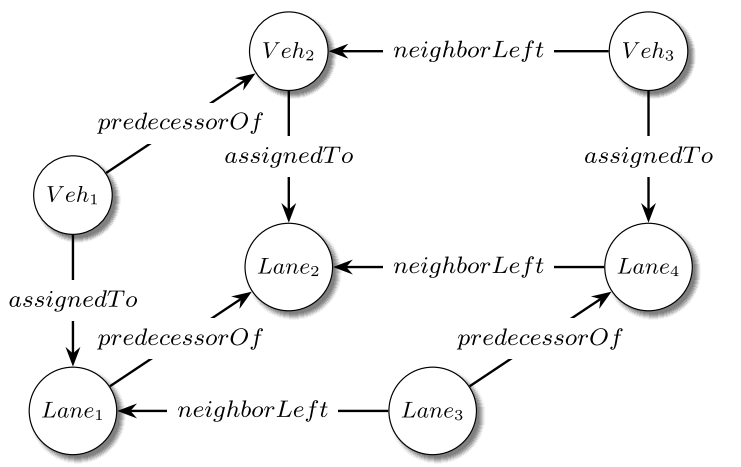
\includegraphics[width=0.7\linewidth]{98_images/relations}
	\caption[Semantic Relations between Traffic Participants]{Illustration of a Graph of Semantic Relations between Traffic Participants \cite{Petrich2018}}
	\label{fig:relations}
\end{figure}

\subsection{Principles of Dynamic World Modeling}
\label{subsec:concept_design:principle_of_dynamic_world_modeling}

\begin{samepage}
	Modeling road traffic requires the ability to capture and integrate perceptual information of highly dynamic environments properly – a problem for which \cite{Crowley1993} states five essential principles. In the following, the original term \textit{"'primitive"'} is substituted by \textit{"'entity"'}. 
	
	\begin{enumerate}[\ \ P1:]
		\item Entities in the world model should be expressed as a \textbf{set of properties}.
		\item Observation and Model should be expressed in a \textbf{common coordinate system}.
		\item Observation and model should be expressed in a \textbf{common vocabulary}.
		\item Properties should include an \textbf{explicit representation of uncertainty}.
		\item Entities should be accompanied by a \textbf{confidence factor}.
	\end{enumerate}
\end{samepage}

This principles are picked up again for the concrete model specification presented later.

\cite{Crowley1993} also presents a "'General Framework for Dynamic World Modeling"', depicted in \autoref{fig:dynamic_world_modeling} (left). It illustrates the high-level process to transform heterogeneous types of observations into a unified model using a common vocabulary. The process includes a \textit{Match-Update-Predict} cycle, the purpose of which is to enhance observations with evidence derived from previous observations and a prediction model. Although especially the \textit{Match} step is quite essential for a real-world system, it is neglected in this thesis for the sake of focusing on the higher-level system architecture. Instead, a simplified process (right) is applied.

Throughout the course of following sections, the above principles are referenced using the respective \textit{\textbf{P}} prefixes.

\begin{figure}
	\centering
	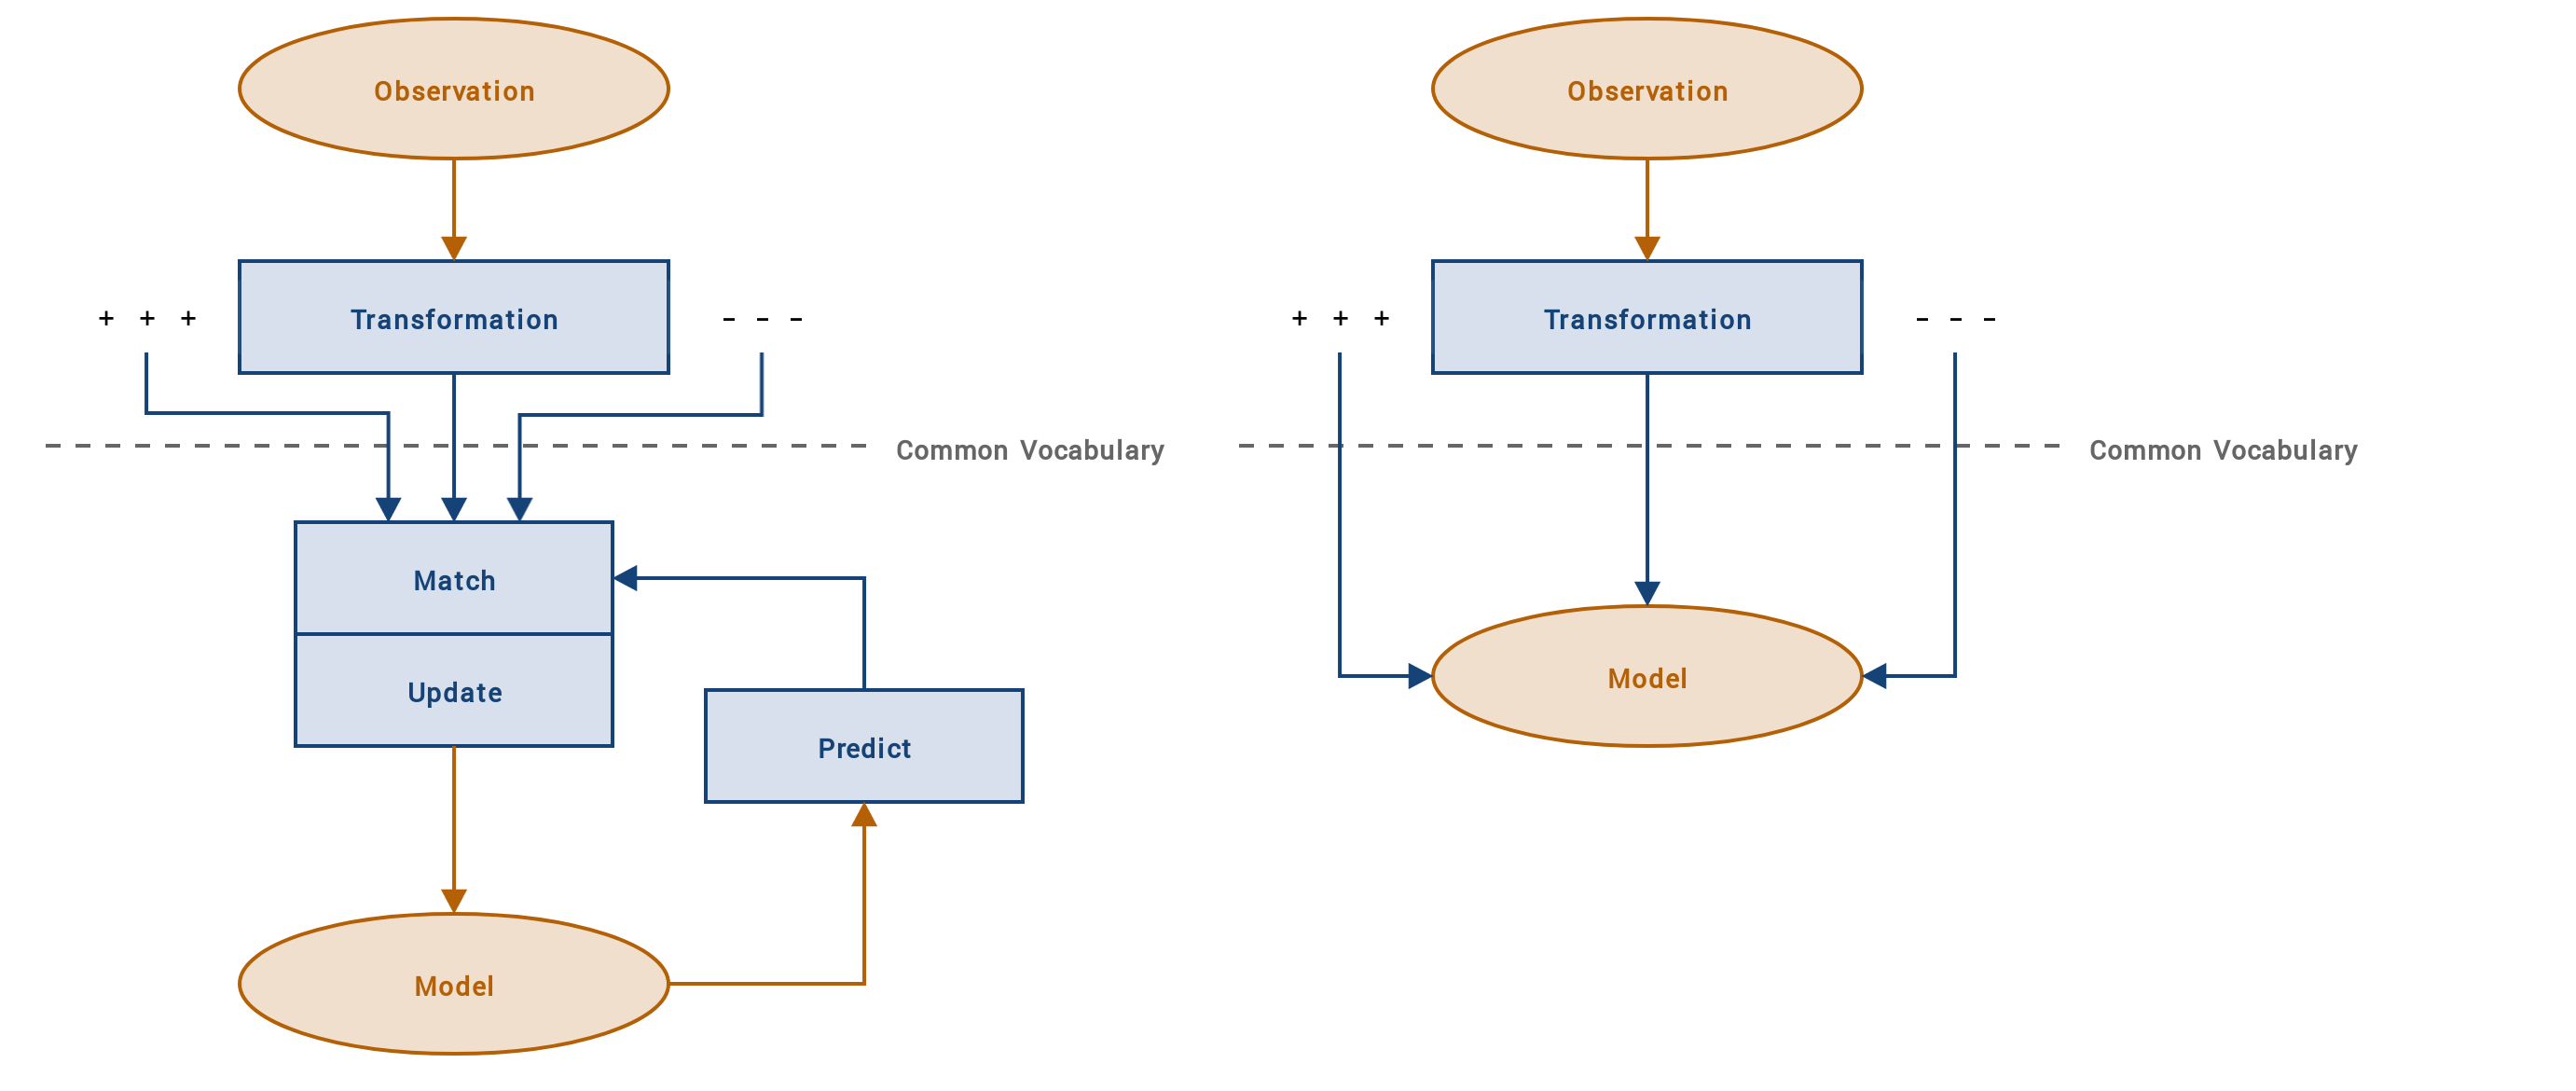
\includegraphics[width=1.0\linewidth]{98_images/dynamic_world_modeling}
	\caption[General Framework for Dynamic World Modeling]{General Framework for Dynamic World Modeling \cite{Crowley1993} (left: original, right: simplified version used in this thesis)}
	\label{fig:dynamic_world_modeling}
\end{figure}

\subsection{Discrete Environment Model with Occupancy Tiles}
\label{subsec:concept_design:discrete_environment_model_with_occupancy_tiles}

When attempting to model one's neighboring traffic environment, a mental distinction can be made into modeling the road network – including lane topology, traffic lights, sidewalks, etc. – and modeling static and dynamic obstacles, like other vehicles, pedestrians or trees. Both aspects are needed for a complete representation, as it is neither sufficient to only know the course of the road nor to only be aware of obstacles. Moreover, it is not sufficient to solely know an obstacle's position, but instead one is usually interested in more advanced properties, too. This work aims to combine all of these aspects in a shared model to enable them for being perceived cooperatively. Accordingly, the idea of \cite{Rauch2011} to share an object list is combined with the concept of \cite{liu2013motion} to share a discretized driveability map, also known as \textit{occupancy grid}. 
\par
\bigskip

The very base of our proposed model is made up of cells of an \textbf{occupancy grid} with fixed dimensions. Such can be constructed by any observer (vehicle, RSU, etc.) and derived from any kind of perceptual sensor data. This simplification facilitates \textbf{universality (NF-M1)}. However, these basic information can be enriched with more complex features easily to support \textbf{expressiveness (F-M1)}. This is achieved through the use of a graph-based meta model, as explained in \autoref{subsec:concept_design:probabilistic_entity_relationship_model_for_traffic_scenes}.

To work towards the \textbf{perspicuity (NF-M2)} requirement and to follow the principle of using a common coordinate system (\textbf{P2}), every cell is identified by a \textbf{QuadKey}. As a consequence, a referring to a cell's position is independent from local, per-vehicle coordinates systems and from the GNSS / GPS coordinate frames alike. This prevents network participants from a multitude of expensive transformation operations.

Following this concept, the entire world map is recursively split into QuadTiles (see \autoref{sec:background:geo_tiling}) of a certain precision level (e.g. level 24, corresponding to square tiles of \textasciitilde\SI{2.39}{\square\meter}). Each cell of the occupancy grid – one of which is observed locally by every connected participant – then corresponds to a certain QuadTile. Besides its occupancy state, every tile can be augmented with information like the corresponding occupant actor, its relation to the overall road topology, etc. 

\autoref{fig:tiling1} illustrates the proposed \textit{occupancy tile} concept. The blue grid is within the observation range of the turquoise vehicle and inherently part of larger tiles. Each cell's (= each tile's) state is determined through local sensor fusion involving different types of sensors and can be extended by additional information. Eventually, that grid, entailing all relevant information, is shared with other CP participants.

\begin{figure}
	\centering
	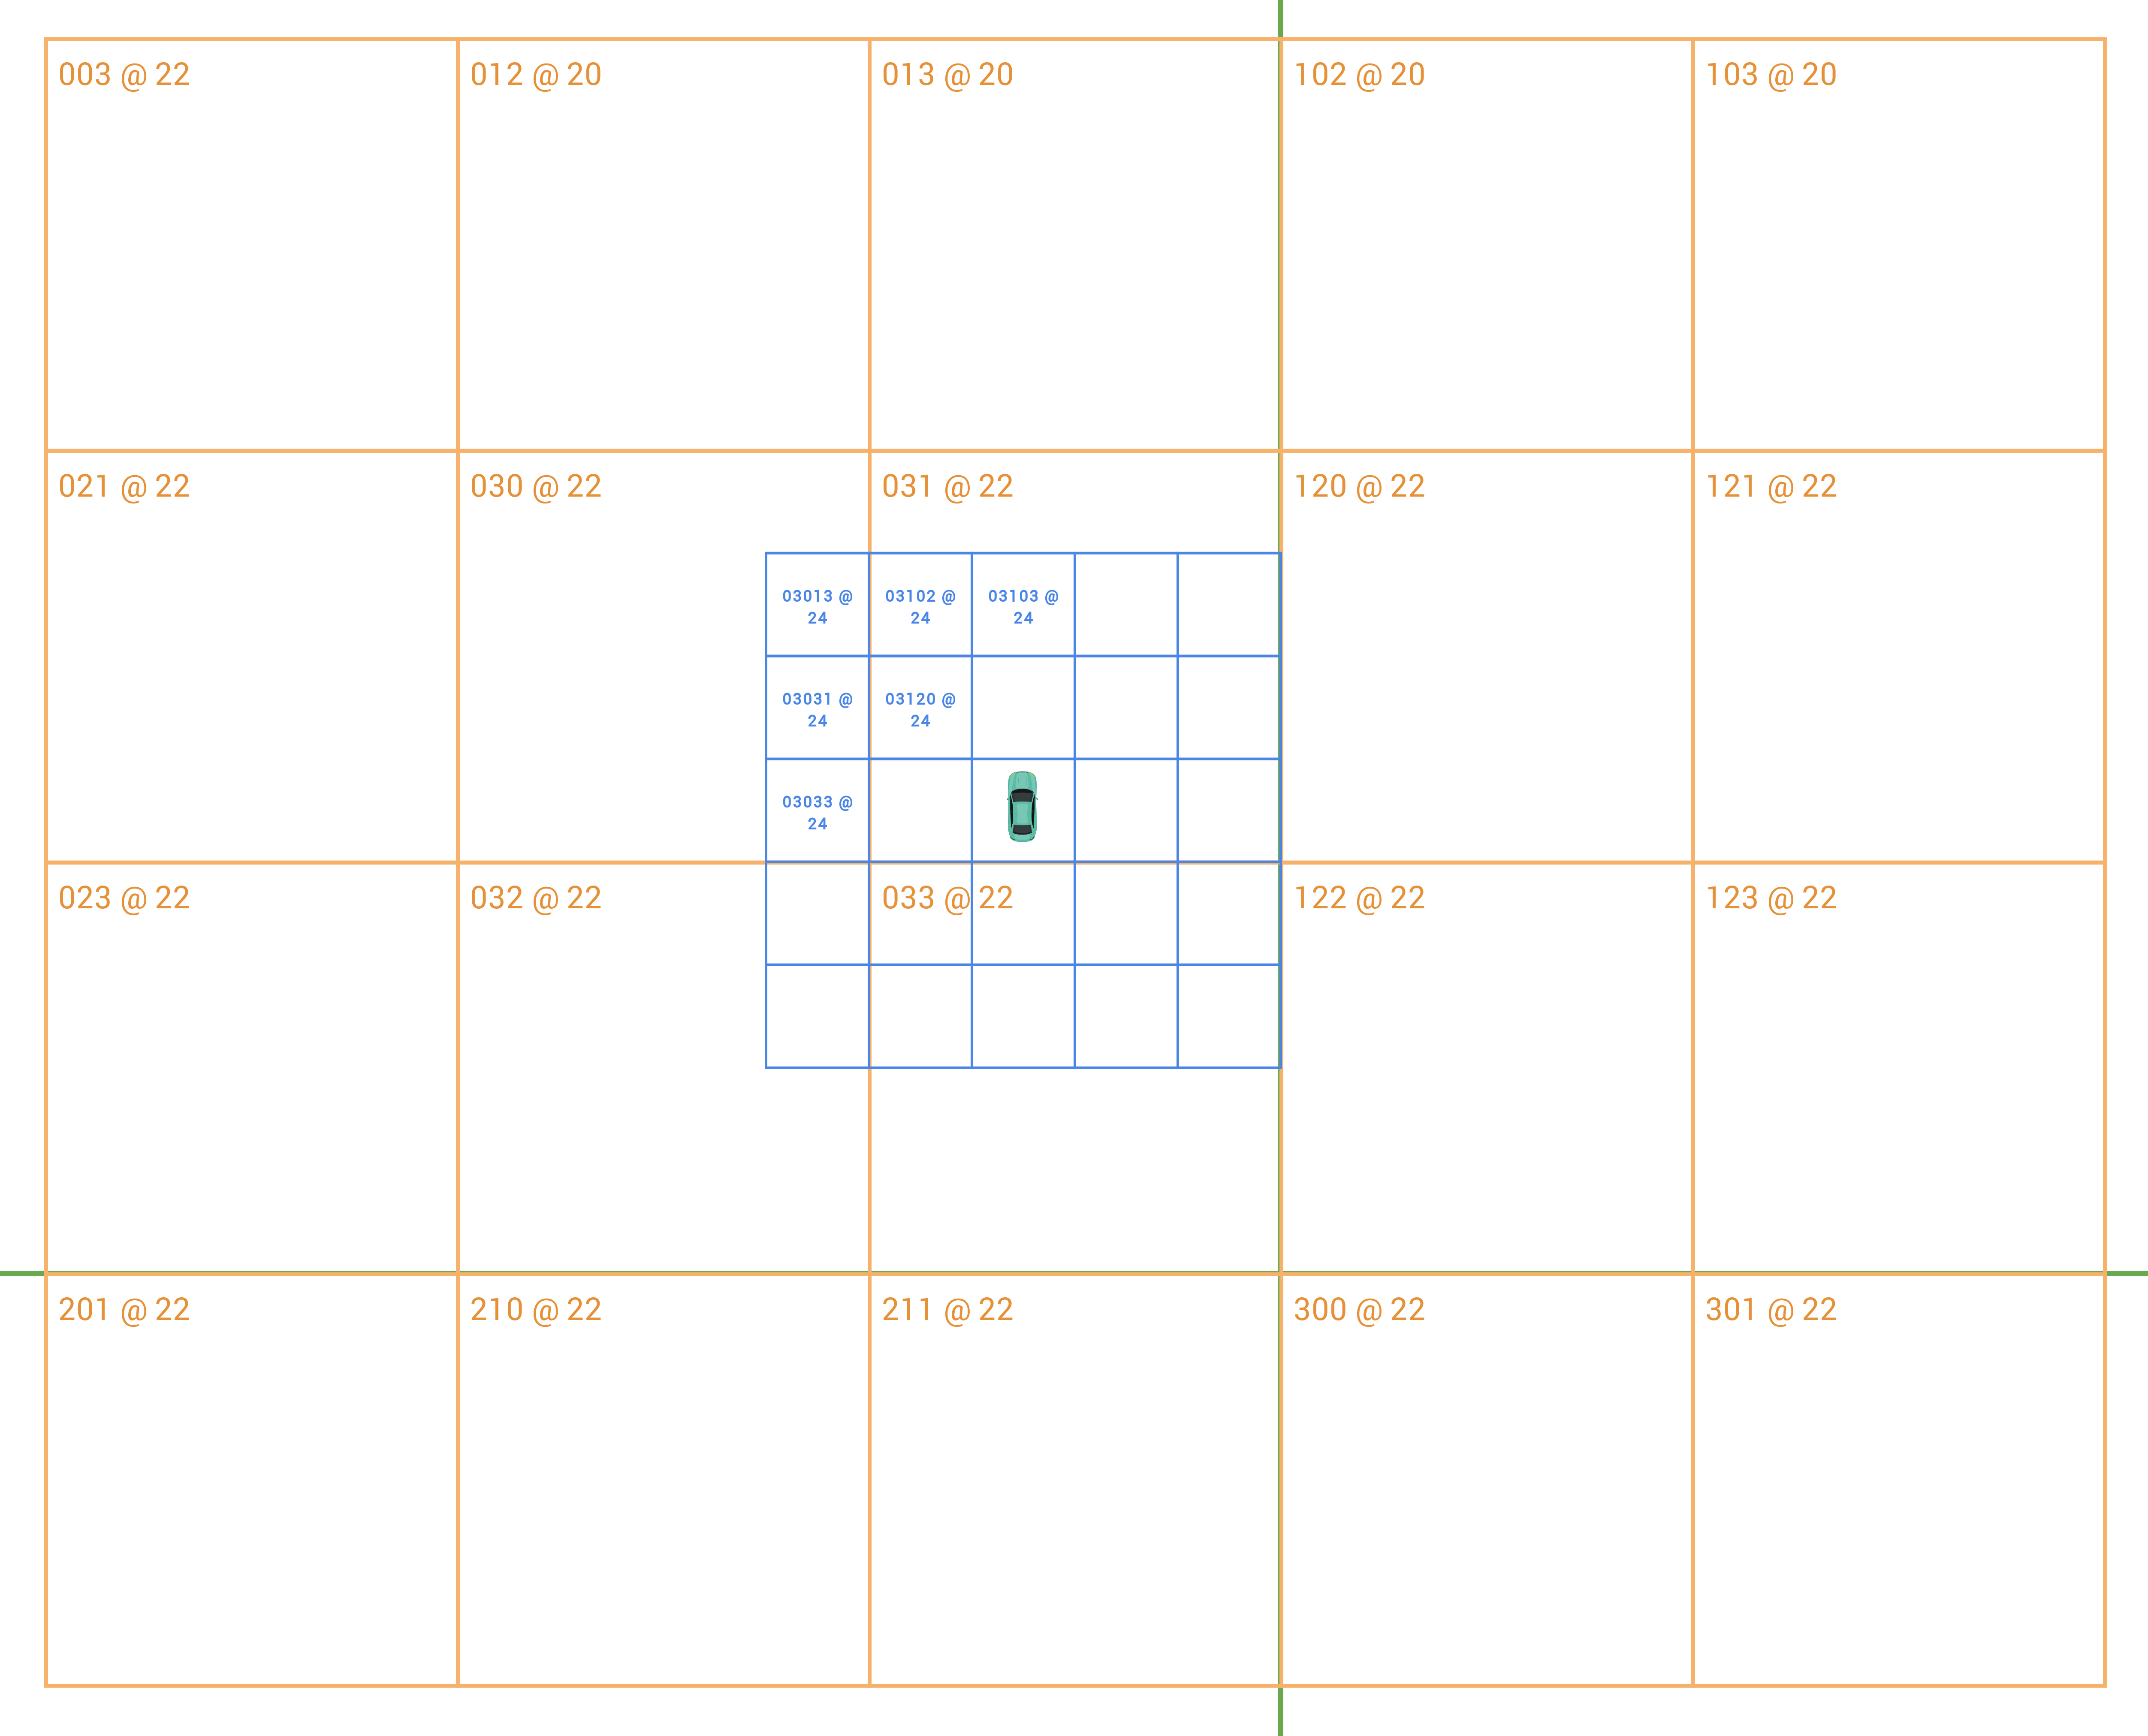
\includegraphics[width=1.0\linewidth]{98_images/geo_subscription_schema_1}
	\caption{Illustration of an Occupancy Grid using QuadTiles}
	\label{fig:tiling1}
\end{figure}


\subsection{Probabilistic Entity Relationship Model for Traffic Scenes}
\label{subsec:concept_design:probabilistic_entity_relationship_model_for_traffic_scenes}